%Jennifer Pan, August 2011

\documentclass[10pt,letter]{article}
	% basic article document class
	% use percent signs to make comments to yourself -- they will not show up.

\usepackage{amsmath}
\usepackage{amssymb}
	% packages that allow mathematical formatting
\DeclareMathOperator*{\argmax}{arg\,max}
\DeclareMathOperator*{\argmin}{arg\,min}
\usepackage{graphicx}
	% package that allows you to include graphics

\usepackage{setspace}
	% package that allows you to change spacing

\onehalfspacing
	% text become 1.5 spaced

\usepackage{fullpage}
	% package that specifies normal margins


\begin{document}
	% line of code telling latex that your document is beginning


\title{ECON500: Problem Set 5}

\author{Nicholas Wu}

\date{Fall 2020}
	% Note: when you omit this command, the current dateis automatically included

\maketitle
	% tells latex to follow your header (e.g., title, author) commands.


\section*{Part 1}
\paragraph{(1.1)}
We first consider the expenditure minimization problem. We present the following lemma:

\textbf{Lemma}: If $u$ is quasilinear in good 1, admits interior solutions, and the price of good 1 is normalized to one, $e(p, u') - e(p, u) = u' - u$.

\textbf{Proof}
Assuming an interior solution, the FOCs are
\[ p_i = \lambda \frac{\partial u}{\partial x_i} \]
Fixing the price of good 1 to be 1, we then have
\[ 1 = \lambda \]
Hence all the prices for goods $i > 1$ must satisfy
\[ p_i = \frac{\partial \tilde{u}}{\partial x_i} \]
Due to constraint binding,
\[ u(h(p,u)) = u \]
\[ \tilde{u}(h_2, h_3, .... h_n) =  u - h_1 \]

Suppose $h'$ is the Hicksian demand at $(p, u')$. Then we know from the FOCs that for $i > 1$,
\[ p_i = \frac{\partial \tilde{u}(h'_2, h'_3, ... ,h'_n)}{\partial x_i} \]
Further, if $h$ is the Hicksian demand at $(p, u)$, we have from the FOCs that for $i > 1$,
\[ p_i = \frac{\partial \tilde{u}(h_2, h_3, ... ,h_n)}{\partial x_i} \]
Hence $h_2, h_3 .... h_{n}$ solves the same system of $n-1$ equations as $h'_2, h'_3, ... h'_n$. Therefore,
$h_i = h'_i$ for $i > 1$. Further, from the constraint binding condition,
\[  h_1 = u - \tilde{u}(h_2, h_3, .... h_n)\]
\[ h'_1 = u' -\tilde{u}(h'_2, h'_3, .... h'_n) \]
\[ h'_1 - h_1 = u' - u \]
Then we have:
\[ e(p, u') - e(p, u)  \]
\[ = \left( p_1 h'_1 + \sum_{i=2}^\infty p_i h'_i \right) - \left( p_1 h_1 + \sum_{i=2}^\infty p_i h_i \right) \]
\[ = p_1 h'_1 - p_1 h_1 \]
\[ = p_1 (h'_1 - h_1)  \]
\[ = u' - u \]
Since the price of good 1 is normalized to 1. $\blacksquare$

Now, our lemma clearly shows that the EV is
\[ e(p^0, u^1) - e(p^0, u^0) = u^1 - u^0 \]
and the CV is
\[ e(p^1, u^1) - e(p^1, u^0) = u^1 - u^0 \]
and hence these are equal. Further, we know that the CS is always between the EV and the CV, so we have that since $EV = CV$, we must have $EV = CS = CV$ as desired.
\paragraph{(1.2)}
Since the sum of the compensating variations is positive, let
\[ \sum_{i=1}^n w_i - e_i(p', v_i(p, w_i)) = k > 0 \]
Define $w'$ as follows. For $i > 1$, let $w'_i = e_i(p', v_i(p,w_i))$. For $i=1$, let
\[ w'_1 = e_1(p', v_1(p, w_1)) + k \]
Then we have
\[ \sum_{i=1}^n w'_i = k + \sum_{i=1}^n e_i(p', v_i(p,w_i)) \]
\[ = \sum_{i=1}^n w_i \]
Now, examine the indirect utility of consumer $i > 1$. Their utility is
\[ v_i(p', w'_i) = v_i(p', e_i(p', v_i(p,w_i)) )  = v_i (p, w_i) \]
So for $i>1$, the consumer neither maintains the same utility level at $w'_i$. Now, for consumer $i=1$, we have
\[ v_i(p', w'_i) = v_i(p', e_i(p', v_i(p,w_i) + k) \ge v_i(p', e_i(p', v_i(p,w_i)) = v_i(p, w_i) \]
and hence consumer 1 is weakly better off. Hence, everyone is weakly better off under $p', w'$ as they were under $p, w$.
\paragraph{(1.3)}
Suppose prices go from $p$ to $p'$ as a result of the excise tax, where $p'_l \neq p$, and $p'_{-l} = p_{-l}$. Then the wealth subsidy that makes the original bundle affordable is given by $\Delta w = (p'_l - p_l) x_l(p, w)$. Then
\[ p'_l x_l(p,w) + \sum_{i \neq l} p'_i x_i(p,w) = (p'_l - p_l) x_l(p,w) + \sum_i p_i x_i(p,w) \le \Delta w + w  \]
Since $x(p,w)$ is affordable at $p', w+\Delta w$, we have by utility maximization that
\[ u(x(p',w+\Delta w)) \ge u(x(p,w)) \]
Now, we note the revenue generated from the excise tax is given by
\[ (p'_l - p_l) x_l(p', w+\Delta w) \]
We note the net revenue to the government is then
\[ (p'_l - p_l) x_l(p', w+\Delta w) - (p'_l - p_l) x_l(p, w) = (p'_l - p_l) (x_l(p', w+\Delta w) - x_l(p, w)) \]
Note that if good $l$ is normal, then typically we will have $x_l(p', w+\Delta w) < x_l(p,w)$, so in order to fully subsidize to the original consumption bundle, the government will be losing money. Hence, the government may not be able to afford to implement this without losing money, so it isn't really a `free lunch'.
\pagebreak
\section*{Part 2}
\paragraph{(2.1)}
\begin{itemize}
\item Homogeneity of degree 1 of $\pi$: \[ \pi(\alpha p) = \max_{y \in Y} \alpha p \cdot y =  \alpha \max_{y \in Y} p \cdot y = \alpha \pi(p) \]
\item Convexity of $\pi$: Let $y$ denote the maximizer correspondence. Then for any $p$, we know $py(p) \ge py(p')$, so
\[ \pi(\alpha p + (1-\alpha)p') = \max_{y \in Y} \left( \alpha p \cdot y + (1-\alpha)p' \cdot y \right) \]
\[ = \alpha p \cdot y(\alpha p + (1-\alpha) p') + (1-\alpha)p' \cdot y(\alpha p + (1-\alpha) p') \]
\[ \le \alpha p \cdot y(\alpha p) + (1-\alpha)p' \cdot y((1-\alpha) p') \]
\[ = \pi(\alpha p) + \pi((1-\alpha)p') \]
\[ = \alpha \pi(p) + (1-\alpha)\pi(p') \]
where we use homogenity in the last step. Hence $\pi$ is convex.
\item Suppose $Y$ is convex. Let $Y' = \{ y \in \mathbb{R}^L: \ py \le \pi(p) \forall p >> 0 \} $. We need to show $Y = Y'$. Consider $y\in Y$. Then by definition of $\pi$, $\pi(p) \ge p\cdot y$ for all $p$. Hence, it is clear that $y \in Y'$, so $Y \subseteq Y'$.

Now, we quickly argue that $Y'$ is convex. Consider $y, y' \in Y'$. Then $\forall p$, $p\cdot y \le \pi(p)$ and $p\cdot y' \le \pi(p)$. This implies for all $p$, $p \cdot \alpha y \le \alpha \pi(p)$ and $p \cdot (1-\alpha) y' \le (1-\alpha) \pi(p)$. Therefore for all $p$, $p \cdot (\alpha y + (1-\alpha)y' ) \le \alpha \pi(p) + (1-\alpha)\pi(p) = \pi(p)$. Hence $\alpha y + (1-\alpha)y' \in Y'$, so $Y'$ is convex.

Having extablished $Y'$ is convex, consider $y' \in Y'$. Suppose, for sake of contradiction, $y' \not \in Y$. Then by the separating hyperplane theorem, since $Y$ is convex, $\exists p$ such that $p \cdot y' > p \cdot y$ for every $y \in Y$. But that implies $p\cdot y' > \pi(p)$, which contradicts the fact $y' \in Y'$. Hence $y' \in Y$, so $Y \subseteq Y'$, so $Y = Y'$.
\item This follows from the fact that multiplying the objective function by a scalar doesn't change the solution to the maximization function:
\[ y(\alpha p) = \arg \max_{y\in Y} \alpha p\cdot y = \arg \max_{y\in Y} p\cdot y = y(p) \]
\item Suppose $Y$ is convex. Consider $y, y' \in y(p)$. Then:
\[ py = py' = \pi(p) \]
So
\[ p\cdot (\alpha y + (1-\alpha)y') = \alpha py + (1-\alpha)py' = \alpha \pi(p) + (1-\alpha)\pi(p) = \pi(p) \]
and since $Y$ is convex, $(\alpha y + (1-\alpha)y') \in Y$. Hence $(\alpha y + (1-\alpha)y') \in y(p)$, so $y(p)$ is convex.

Now, suppose $Y$ is strictly convex, and $y \neq y' \in y(p)$. We have
\[ p\cdot (\alpha y + (1-\alpha)y') = \alpha py + (1-\alpha)py' = \alpha \pi(p) + (1-\alpha)\pi(p) = \pi(p) \]
But since $Y$ is strictly convex, $\alpha y + (1-\alpha)y'$ is in the interior of $Y$, and hence $\exists$ some neighborhood $B(\alpha y + (1-\alpha)y', \epsilon) \subset Y$ (supposing we are under the sup norm). This implies $y'' = \alpha y + (1-\alpha)y' + (\epsilon)\vec{1} \in Y$. But that means that $p\cdot y'' = p \cdot (\alpha y + (1-\alpha)y') + \epsilon p \cdot \vec{1} = \pi(p) + \epsilon p\cdot \vec{1} > \pi(p)  $, which is a contradiction of the definition of $\pi$. Hence, it is impossible for $y \neq y'$, and hence $y = y'$. So $y(p)$ is single-valued.
\item Assuming the right differentiability conditions, (i.e. $y$ singleton, $\pi$ differentiable) then we have that since $y$ is the maximizer of the maximization problem whose value is $\pi$, by the envelope theorem
\[ \frac{\partial \pi}{\partial p_l} = y_l - \lambda \frac{\partial g}{\partial p_l} \]
where $g$ encapsulates the feasible set constraints. However, the feasible set has no dependence on $p$, so the term is 0, and hence
\[ \frac{\partial \pi}{\partial p_l} = y_l \]
\item If $D_py(p)$ does not exists, this statement is vacuously true. Supposing $y$ is singleton and differentiable so $Dy$ exists, by Hotelling's lemma,
\[ y = D \pi \]
\[ Dy = D^2 \pi \]
By Young's theorem, $D^2 \pi$ is symmetric, so by Hotelling, $Dy$ is symmetric. Further, since $\pi$ is convex, $D^2 \pi$ is positive semidefinite, so from Hotelling, $Dy$ is positive semidefinite.

Finally, by homogeneity of degree 0 for $y$, we have
$y(\alpha p) = y(p)$. Differentiating with respect to $\alpha$, we get
\[ D_{\alpha p} y(\alpha p) \cdot D_\alpha {\alpha p} = 0 \]
\[ D_p y(p) \cdot p = 0 \]
\end{itemize}
Now we consider the cost function $c(w,q)$ and input demand function $z(w, q)$.
\begin{itemize}
\item This follows from the fact that multiplying the objective function by a scalar doesn't change the solution to the minimization problem:
\[ c(\alpha w, q) = \min_{f(z) \ge q} \alpha w \cdot z =  \alpha \min_{f(z) \ge q}  w \cdot z = \alpha c(w, q) \]
\item Let $q' > q$. Then $c(w, q') = w \cdot z(w, q')$. We then know that since $f(z(w, q')) \ge q' > q$, $z(w,q')$ is in the feasible set for the minimization problem at $(w, q)$, so
\[\min_{f(z) \ge q}  w \cdot z \le w \cdot z(w, q') \]
\[ c(w, q) \le c(w, q') \]
And hence $c$ is increasing in $q$.
\item Let $Y' = \{ (-z, q) : \ wz \ge c(w,q) \forall w >> 0 \}$. Let $(-z, q) \in Y$. Then by definition of $Y$, $q \le f(z)$, so $z$ is feasible for the the minimization problem at $w,q$ for all $w$. Hence $c(w, q) \le w \cdot z$ for all $w$, so $(-z, q) \in Y'$. Hence $Y \subseteq Y'$.

Now, suppose $(-z, q) \in Y'$. Suppose, for sake of contradiction, that $f(z) < q$. Consider the set $S_q = \{z : \ f(z) \ge q \}$ Then $z \not \in S_q$, and by our supposition, $S_q$ is convex, so by the separating hyperplane theorem, there exists some $w$ such that $w \cdot z < w \cdot z'$ for all $z' \in S_q$. Then since $z(w, q) \in S_q$, $w \cdot z < w \cdot z(w,q) = c(w, q)$. This is a contradiction of the fact $(-z, q) \in Y'$, so we must have $f(z) \ge q$. Hence $(-z, q) \in Y$, so $Y' \subseteq Y$. So $Y = Y'$.
\item Consider $z, z' \in z(w,q)$. Then we know
\[ w z = wz' = c(w, q) \]
Hence
\[ w(\alpha z + (1-\alpha) z') = \alpha w z + (1-\alpha) w z' = c(w,q) \]
By the necessary convexity, $f(\alpha z + (1-\alpha) z') \ge q$, so $\alpha z + (1-\alpha)z' \in z(w,q)$. Hence $z(w,q)$ is convex. Now, suppose the sets $S_q = \{ z | f(z) \ge q \}$ are strictly convex. Suppose, for sake of contradiction, $z \neq z' \in z(w,q)$. Then by strict convexity, $\alpha z + (1-\alpha)z'$ is in the interior of $S_q$, implying that there exists some $\epsilon$ neighborhood (take the sup norm) of $\alpha z + (1-\alpha) z' $ that is contained in $S_q$. This implies that
\[ f( \alpha z + (1-\alpha)z' - \epsilon \vec{1}) \ge q \]
But that implies
\[ w\cdot( \alpha z + (1-\alpha)z' - \epsilon \vec{1}) = \alpha wz + (1-\alpha)wz' - \epsilon w\cdot 1 = c(w,q)- \epsilon w\cdot 1 < c(w,q)   \]
But this contradicts the definition of $c(w,q)$ as the minimization of $wz$ such that $f(z) \ge q$, so we cannot have $z \neq z'$. Hence $z(w,q)$ must be single-valued.
\item Fix a sequence $w^n \to w$, where the sequence fixes $w_{-l}$. Consider the sequence $d^n = \frac{c(w^n, q) - c(w, q)}{w^n_l - w_l}$. We want to show $d^n \to z_l(w, q)$. Note that
\[ d^n = \frac{w^n_l z_l(w^n_l, w_{-l}, q) + \sum_{i \neq l} w_i z_i(w^n_l, w_{-l}, q)  - w_l z_l(w_l, w_{-l}, q) - \sum_{i \neq l} w_i z_i(w_l, w_{-l}, q)}{w^n_l - w_l} \]
\[ = \frac{w^n_l z_l(w^n_l, w_{-l}, q)- w_l z_l(w_l, w_{-l}, q) + \sum_{i \neq l} w_i (z_i(w^n_l, w_{-l}, q) - z_i(w_l, w_{-l}, q))}{w^n_l - w_l} \]
Then
\[ d^n - z_l(w,q) = \frac{w^n_l z_l(w^n_l, w_{-l}, q)- w_l z_l(w, q) + \sum_{i \neq l} w_i (z_i(w^n_l, w_{-l}, q) - z_i(w, q))}{w^n_l - w_l} - \frac{w^n_lz_l(w,q) - w_l z_l(w,q)}{w^n_l - w_l} \]
\[ = \frac{w^n_l (z_l(w^n_l, w_{-l}, q)-  z_l(w, q)) + \sum_{i \neq l} w_i (z_i(w^n_l, w_{-l}, q) - z_i(w, q))}{w^n_l - w_l} \]\[ = \frac{(w^n_l - w_l) (z_l(w^n_l, w_{-l}, q)-  z_l(w, q)) + \sum_{i} w_i (z_i(w^n_l, w_{-l}, q) - z_i(w, q))}{w^n_l - w_l} \]
\[ = (z_l(w^n_l, w_{-l}, q)-  z_l(w, q)) + \frac{ \sum_{i} w_i (z_i(w^n_l, w_{-l}, q) - z_i(w, q))}{w^n_l - w_l} \]
\[ \ge (z_l(w^n_l, w_{-l}, q)-  z_l(w, q)) \]
since $w \cdot z(w^n_l, w_{-l}, q) \ge w \cdot z(w,q)$. Further
\[d^n - z_l(w,q) = \frac{w^n_l (z_l(w^n_l, w_{-l}, q)-  z_l(w, q)) + \sum_{i \neq l} w_i (z_i(w^n_l, w_{-l}, q) - z_i(w, q))}{w^n_l - w_l} \]
\[ =  \frac{w^n_lz_l(w^n_l, w_{-l}, q)+ \sum_{i \neq l} w_i z_i(w^n_l, w_{-l}, q)-  w^n_l z_l(w, q) - \sum_{i \neq l} w_i z_i(w^n_l, w_{-l}, q) }{w^n_l - w_l} \]
\[ = \frac{w^n \cdot z(w^n, q) - w^n \cdot z(w,q)}{w^n_l - w_l} \]
\[ \le 0 \]
Since $w^n \cdot z(w^n, q) \le w^n \cdot z(w,q)$. So we have
\[ 0 \ge d^n - z_l(w,q) \ge (z_l(w^n_l, w_{-l}, q)-  z_l(w, q)) \]
HSince $z$ must be upper hemicontinuous and is single-valued, $z$ is continuous, and hence the RHS converges to 0. Therefore, $d^n - z_l(w,q) \to 0$, so $d^n  \to z_l(w,q)$. Hence $c$ is differentiable, and
\[ \frac{\partial c(q, w)}{\partial w_l} = z_l(w,q) \]
\item From the previous result, we have
\[ D_w c(w,q) = z \]
\[ D_w^2 c(w,q) = D_wz \]
By Young's theorem, this is symmetric. To show this is negative semidefinite, we show that $c(w,q)$ is concave in $w$. Consider $w, w', q$. Then since $w z \le c(w,q)$ for $f(z) \ge q$.
\[ c(\alpha w + (1-\alpha)w', q) = \alpha w z(\alpha w + (1-\alpha)w', q) + (1-\alpha) w' z(\alpha w + (1-\alpha)w', q) \]
\[ \le \alpha w z(w, q) + (1-\alpha) w' z(w', q)  \]
\[ = \alpha c(w,q) + (1-\alpha)c(w', q) \]
Hence $c$ is concave in $w$, so $D^2_w c $ is negative semidefinite.
Now, since $c$ is homogeneous of degree 1, we have
\[ c(\alpha w, q) = \alpha c(w,q) \]
\[ \alpha w \cdot z(\alpha w, q) = \alpha w \cdot z(w,q)\]
\[ w \cdot z(\alpha w, q) = w \cdot z(w,q) \]
Since this holds for all $w$, we get
\[ z(\alpha w, q) = z(w,q) \]
Differentiating both sides wrt $\alpha$, we get
\[ \sum_{i=1}^L \frac{\partial z_i(\alpha w, q)}{\partial (\alpha w_i)} \frac{\partial (\alpha w_i)}{\partial \alpha} = 0\]
\[ \sum_{i=1}^L w_i \frac{\partial z_i(w, q)}{\partial w_i} = 0\]
\[ D_w z \cdot w = 0 \]
\item Suppose $f$ is homogeneous of degree 1. Consider
\[ c(w, \alpha q) = \min_{f(z) \ge \alpha q} w \cdot z = \min_{\frac{1}{\alpha}f(z) \ge q} w \cdot z = \min_{f(z/\alpha) \ge q} \alpha w \cdot (z/\alpha)= \alpha \min_{f(z/\alpha) \ge q} w \cdot (z/\alpha) = \alpha c(w,q) \]
Now,
\[ z(w, \alpha q) = \arg\min_{f(z) \ge \alpha q} w \cdot z = \arg\min_{\frac{1}{\alpha}f(z) \ge q} w \cdot z = \arg\min_{f(z/\alpha) \ge q} w \cdot (z/\alpha)= \alpha \arg\min_{f(z) \ge q} w \cdot z = \alpha c(w,q) \]
\item Let $f$ be concave. Consider $q, q'$. We know that
\[ f(z(w,q)) \ge q \]
\[ f(z(w,q')) \ge q' \]
By concavity,
\[ f(\alpha z(w,q) + (1-\alpha)z(w,q')) \ge \alpha f(z(w,q)) + (1-\alpha)f(z(w,q')) \ge \alpha q + (1-\alpha)q' \]
So therefore
\[ \alpha c(w,q) + (1-\alpha)c(w,q') = \alpha w \cdot z(w,q) + (1-\alpha) w \cdot z(w,q') \]
\[ = w \cdot (\alpha z(w,q) + (1-\alpha)z(w,q')) \]
\[ \ge w \cdot z(w, \alpha q + (1-\alpha) q') \]
\[ = c(w, \alpha q + (1-\alpha) q') \]
and so $c$ is convex in $q$.
\end{itemize}
\paragraph{(2.2)}
The comparative statics for Marshallian demands are:
\[ \frac{\partial x_i}{\partial p_i},\frac{\partial x_i}{\partial p_j},\frac{\partial x_i}{\partial w} \]
We know from our previous psets that the signs of all of these are ambiguous. For Hicksians,
\[ \frac{\partial h_i}{\partial p_i},\frac{\partial h_i}{\partial p_j}\]
We know that the own-effect term $\partial h_i / \partial p_i$ is negative, since the Slutsky matrix is negative semidefinite. The other terms can have any sign.

Now, for the firm problem:
\[ \max p_1 y_1 + p_2 y_2 + p_3 y_3 \]
subject to
\[ y_1 = f(-y_2, -y_3)\]
where we assume that net production of inputs is negative and production of the output is positive. Now, from $2.1$, we established that $Dy(p)$ is positive semidefinite. Hence, when we examine comparative statics
\[ \frac{\partial y_i}{\partial p_i}, \frac{\partial y_i}{\partial p_j} \]
we know that the diagonal entries, or the own-effects, are positive. That is,
\[ \frac{\partial y_i}{\partial p_i} > 0 \]
The signs of the non-diagonal entries are ambiguous. For the input demands $z(w,q)$, we established in $2.1$ that $D_w z$ is negative semidefinite. Hence, we have that
\[ \frac{\partial z_i}{ \partial w_i} < 0 \]
The other off-diagonal entries have ambiguous signs.

\paragraph{(2.3)}
We note that changing prices for the firm's profit maximization problem changes only the objective function, which means that increasing the price of something implies that since the original maximizer is still feasible, the new maximizer should be weakly increasing in the price (for an input, the firm uses less of the input since it increases towards 0). However, in the utility maximization problem, increasing price changes the feasible region of the problem, and therefore it is possible for an increase in price to increase consumption.
\paragraph{(2.4)}
\begin{itemize}
\item We clearly see that $c$ is not convex in $q$: the second derivative is $6q-20$, which is negtive for $q=1$, for example. Hence, from the last part of 2.1, we know $f$ cannot be a concave production function, which then implies that our production set is not convex.
\item See figures 1 and 2.
\begin{figure}
\centering
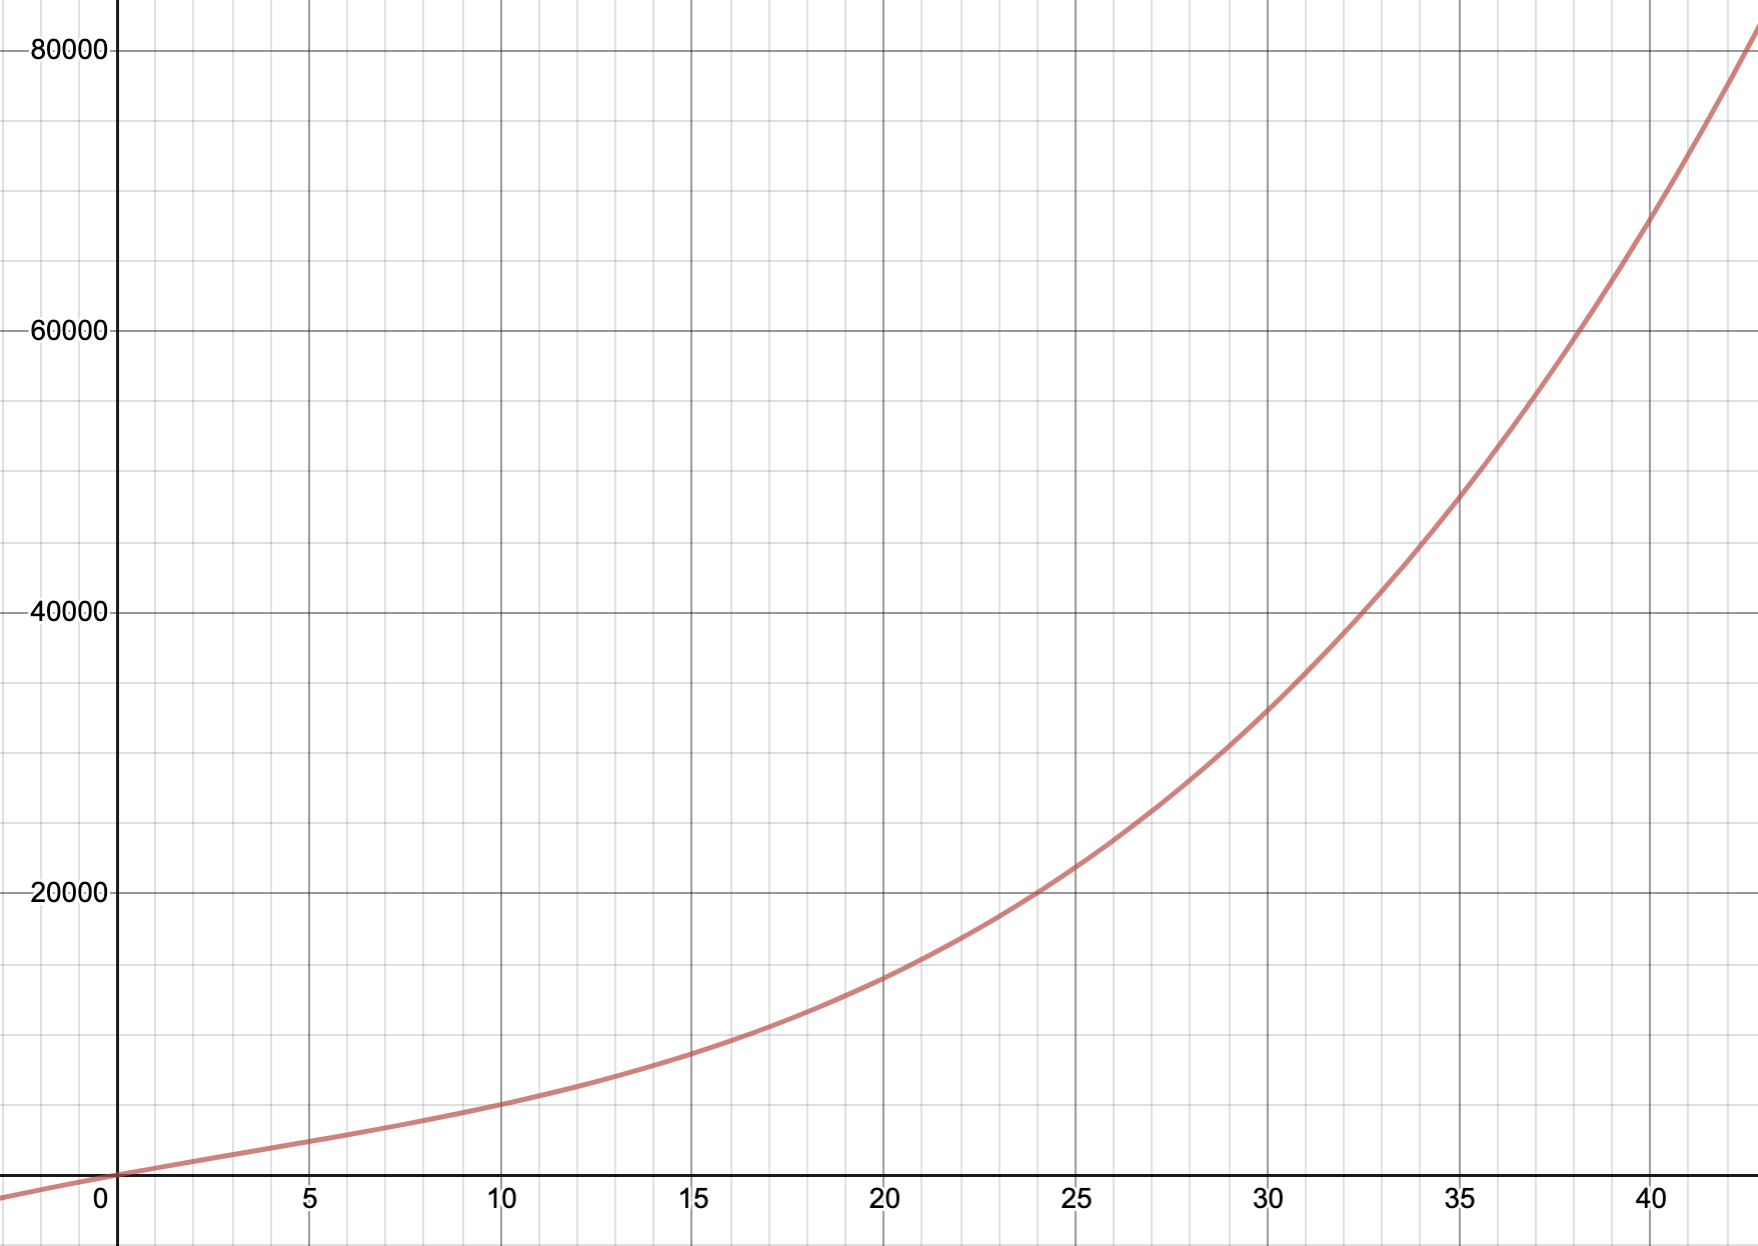
\includegraphics[scale=0.4]{ps5fig1}
\caption{Total cost, 2.4.b}
\end{figure}
\begin{figure}
\centering
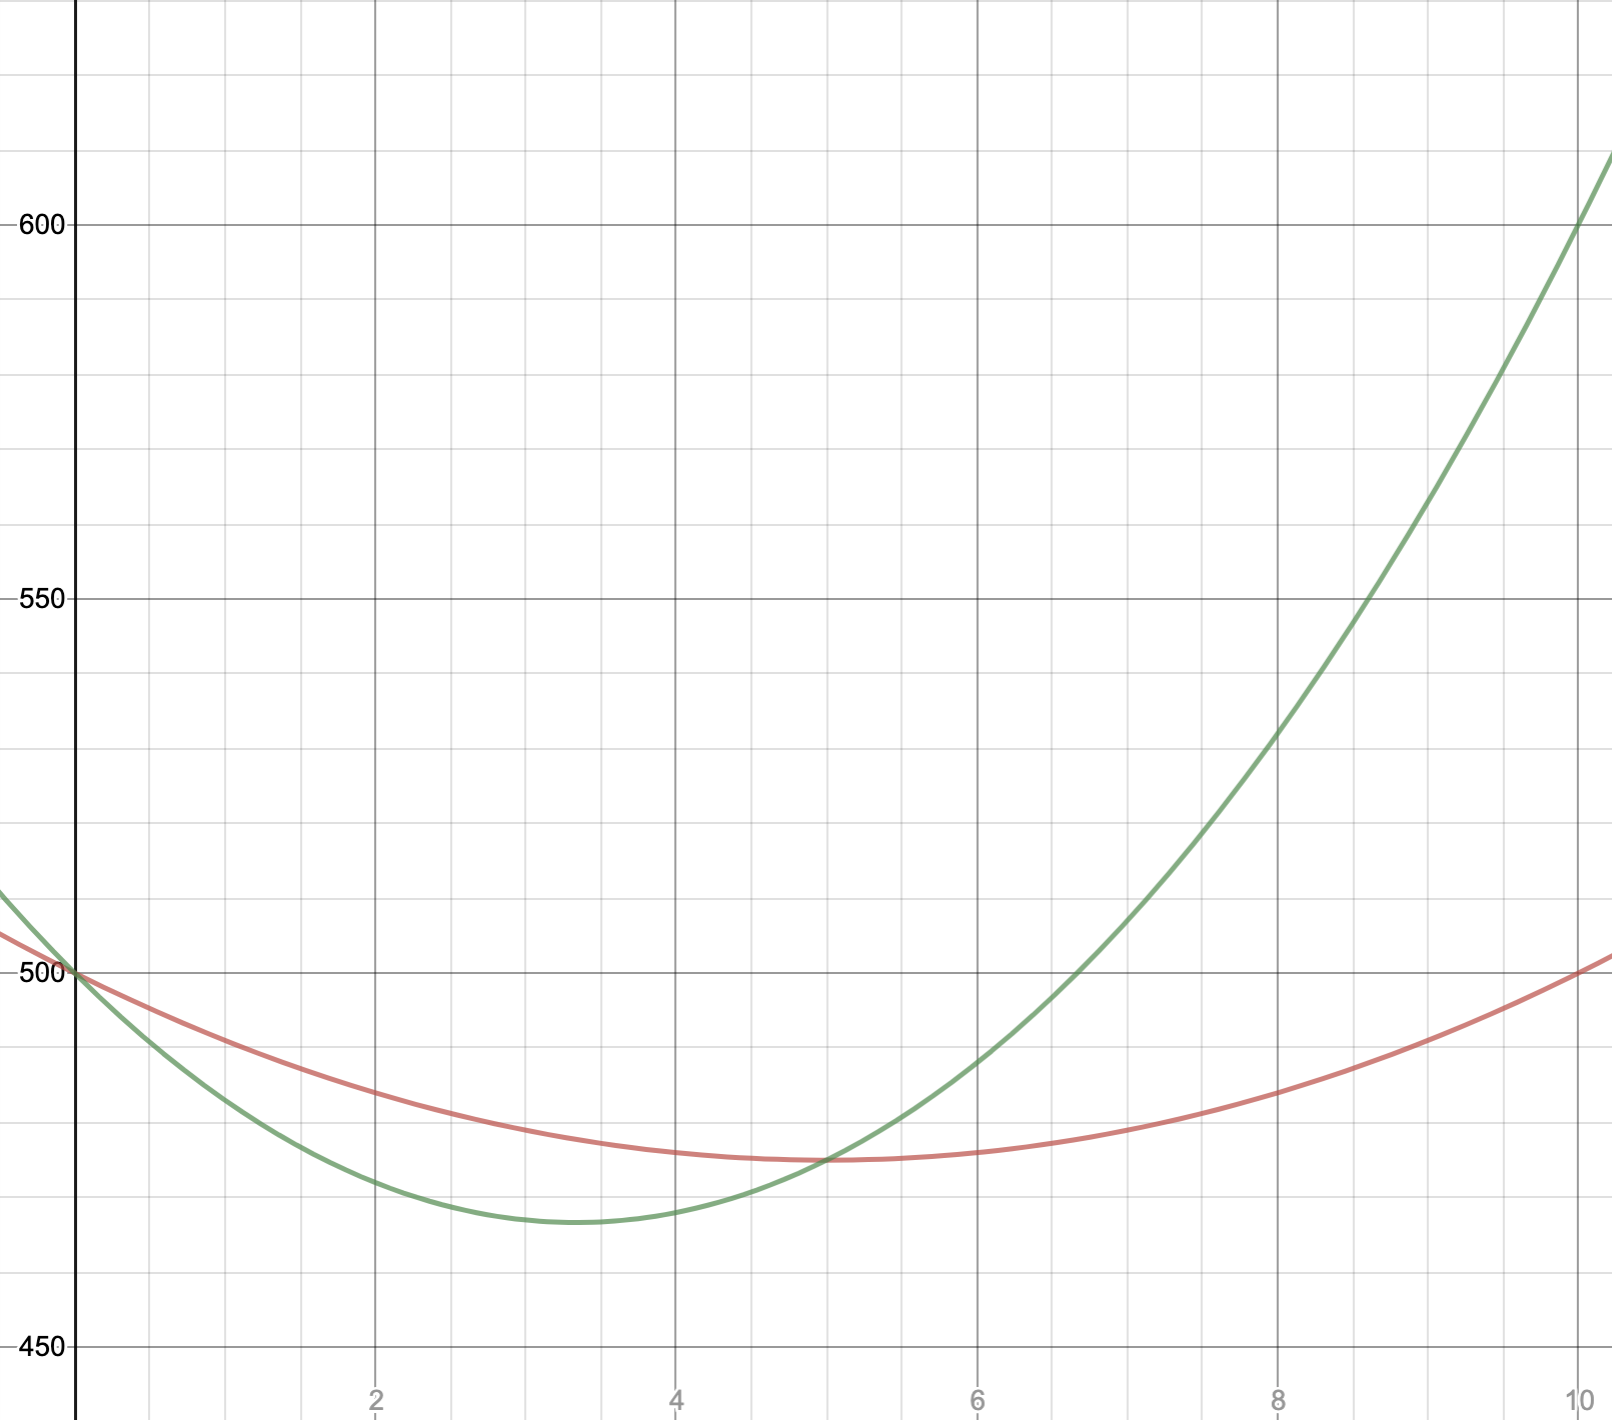
\includegraphics[scale=0.4]{ps5fig2}
\caption{Average and marginal cost, 2.4.b. Average cost in red, marginal cost in green.}
\end{figure}
\begin{figure}
\centering
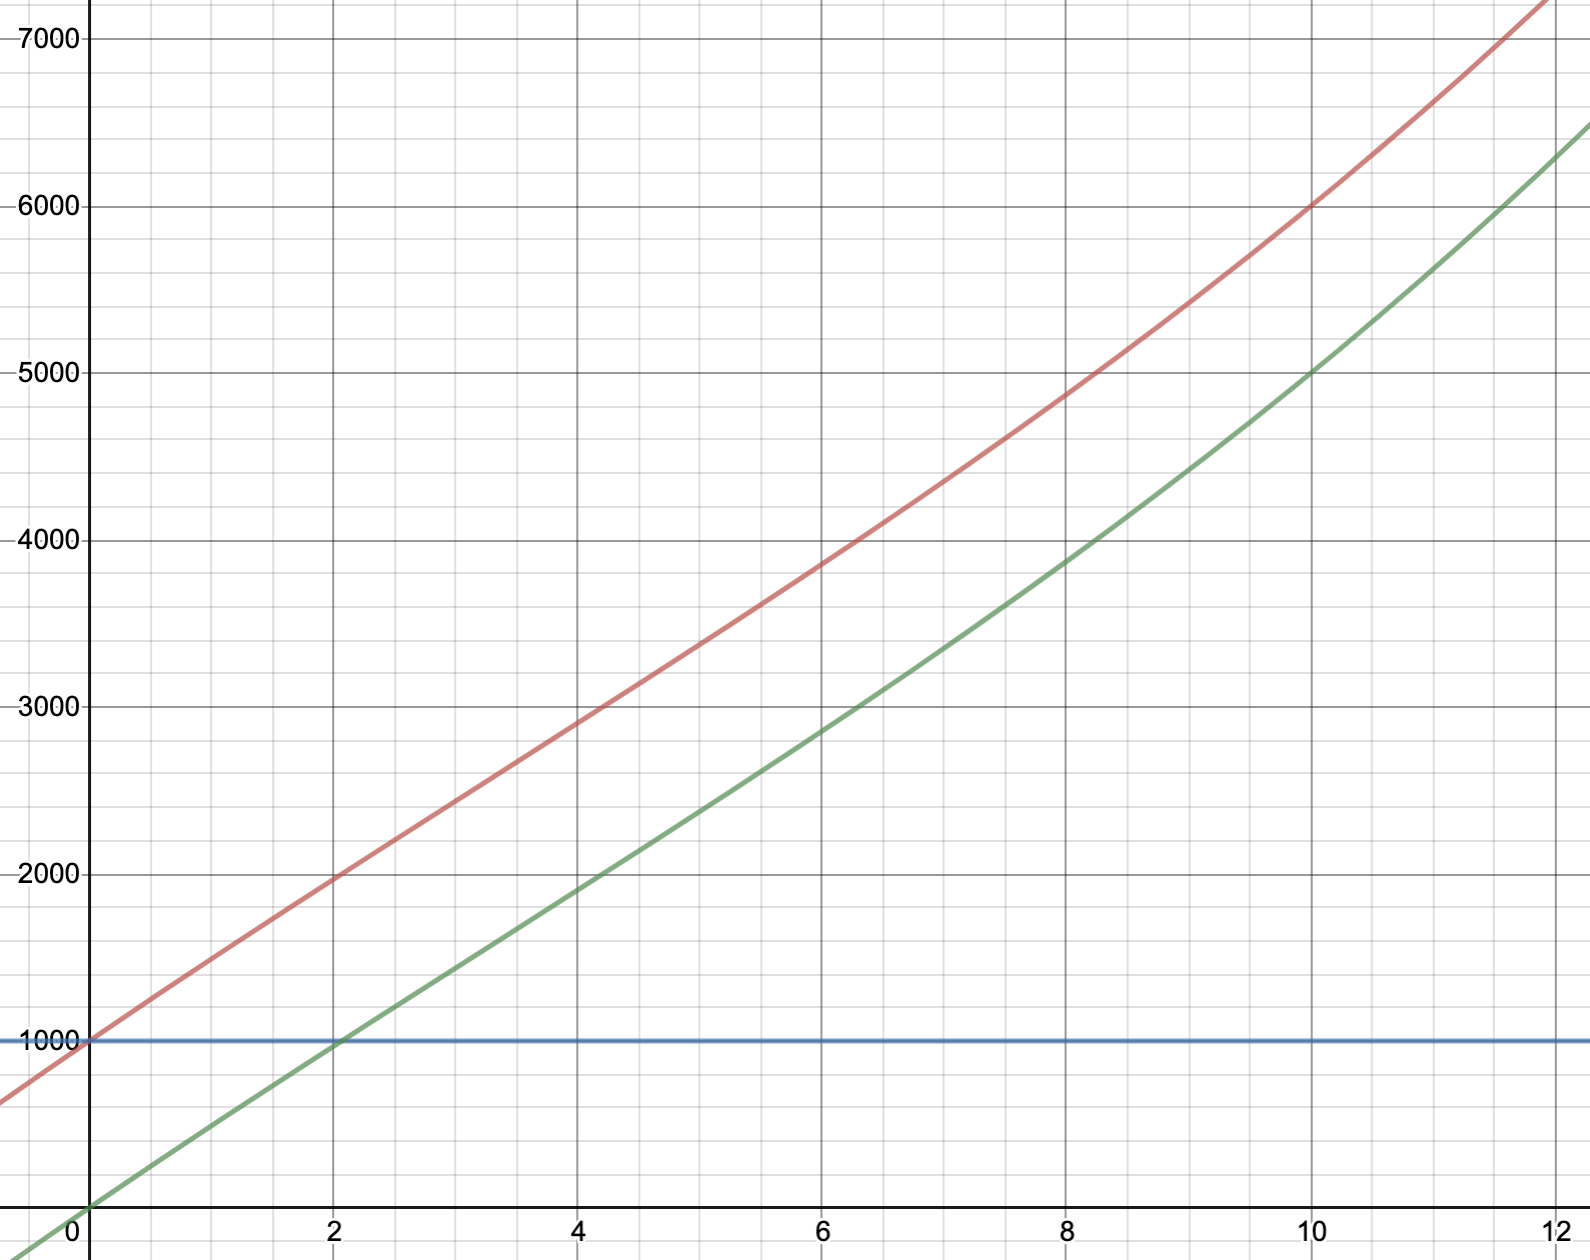
\includegraphics[scale=0.4]{ps5fig3}
\caption{Total cost, variable cost, fixed cost, 2.4.c. Total cost in red, fixed cost in blue, variable cost in green.}
\end{figure}
\begin{figure}
\centering
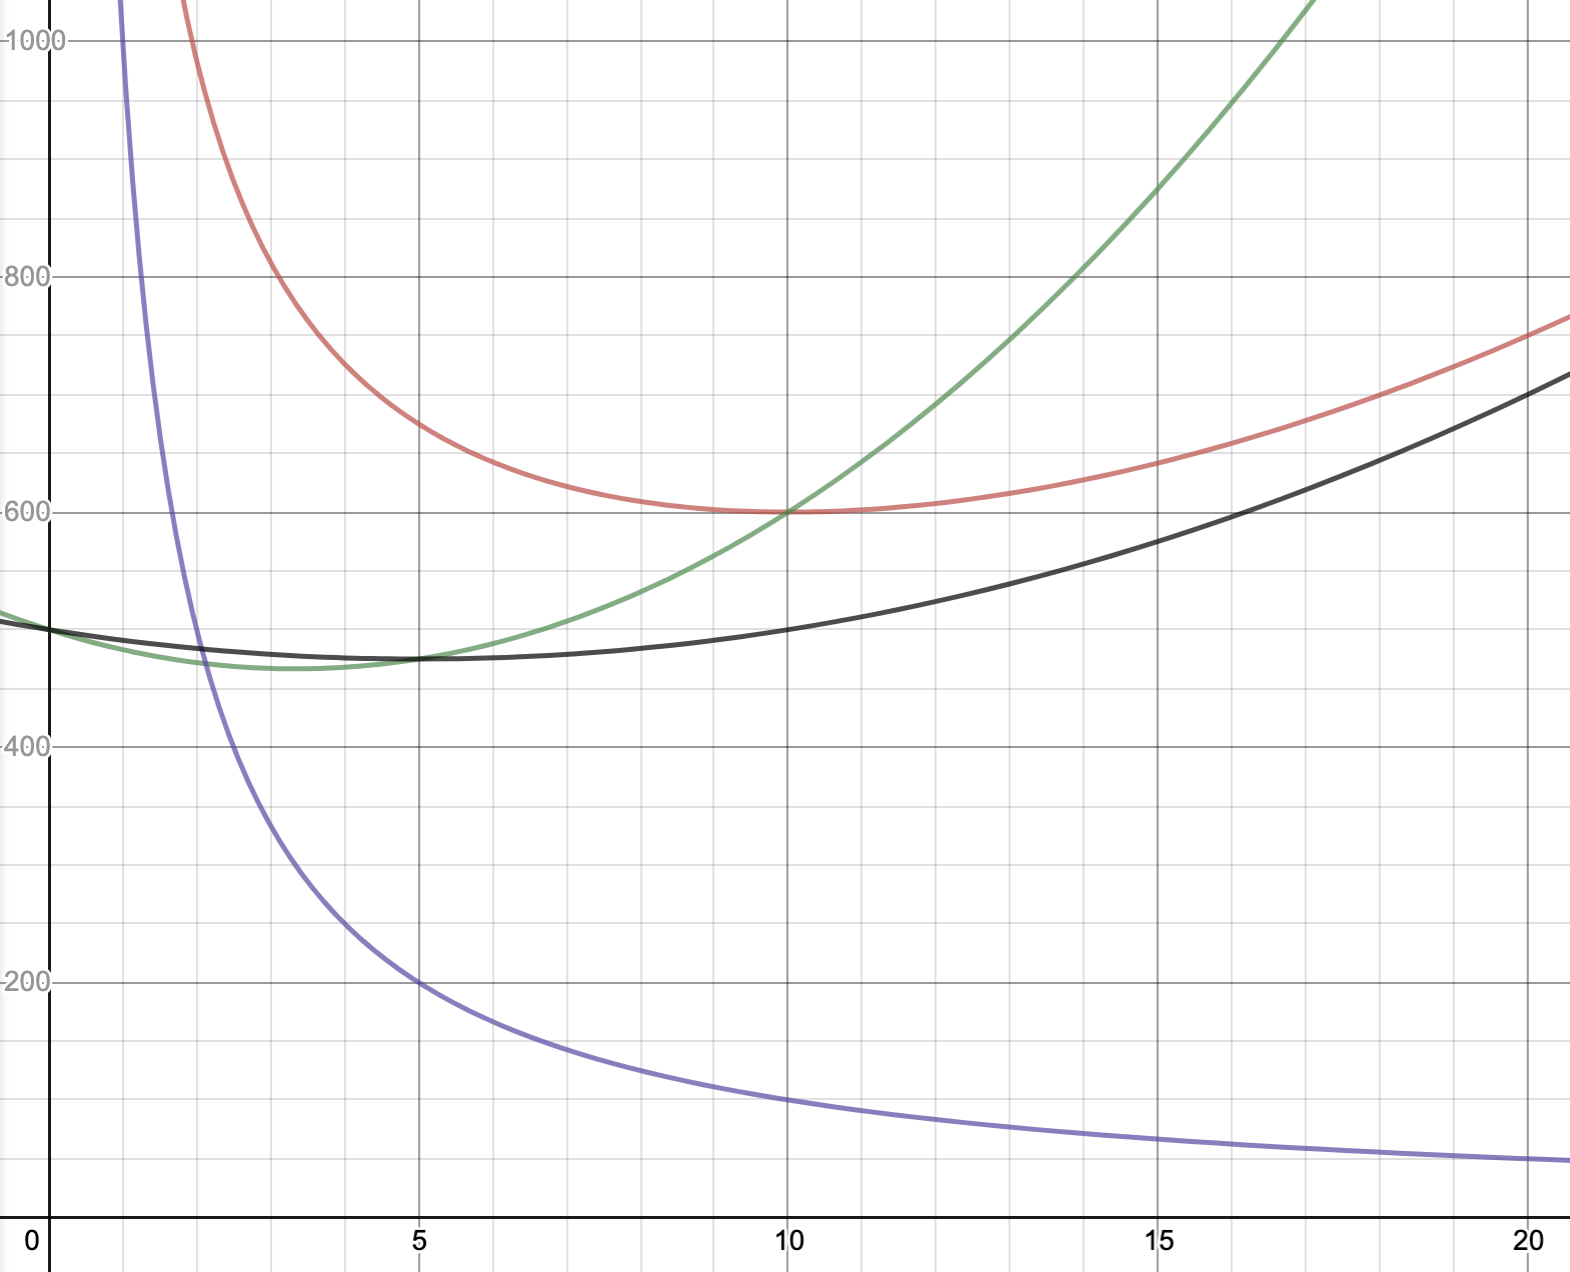
\includegraphics[scale=0.4]{ps5fig4}
\caption{Average cost, average variable cost, average fixed cost, and marginal cost, 2.4.c. Average cost in red, marginal cost in green, average variable cost in black, average fixed cost in purple.}
\end{figure}
\item See figures 3 and 4.
\item The firm seeks to maximize:
\[ \pi(p) = \max_q pq - C(q) \]
We first note that if $p < 600$, the firm's profit is weakly negative, so the firm will always take $q=0$ in this case. If $p = 600$, the firm is indifferent between producing $q=0$ and $q=10$, (both have 0 profit). For $p > 600$, we have
This has the FOC:
\[ p = 500 - 20q + 3q^2 \]
\[ 3q^2 - 20q + (500-p) = 0 \]
At equilibrium, we will have:
\[ p = 10600 - nq \]
Taking $p = 600$ and $q = 10$, we find $n=1000$. The net quantity is then $Q = nq = 10000$. Note that in this equilibrium, firms produce $q=10$ at price $600$, so their profit is $6000 - (1000 + 5000 - 1000 + 1000) = 0$.
\item Millicent's proposed function becomes very negative for large $q$. If we take $q = 100$, we would find a cost of
\[50000 - 100000 = -50000 \]
and hence we would love to just produce $\infty$ amount of $q$ to generate arbitrarily large profits.
\item For the graphs, see figures 5 and 6. The marginal and average cost functions are linear now, and the total cost is convex. The FOC is then:
\[ p = 500 + 20q \]
\[ q = (p/20) - 25 \]
Assuming the same demand function,
\[ p = 10600 - nq \]
\[ p/20 = 530 - (nq)/20 \]
\[ 505 = q (n+20)/20 \]
\[ 10100/q - 20 = n \]
In the long run case, we then have that sinze profits tend to 0,
\[ (500  + 20q) q - (500q + 10q^2) = 0 \]
\[ q \to 0 \]
 Therefore, $n\to \infty$, $nq \to 10100 $ and $p \to 500$. So we have an infinite number of firms, producing 0 each for a net production of $10100$, and price $500$. Millicent might be concerned about having infinite firms, or 0 output per firm, or both.
\begin{figure}
\centering
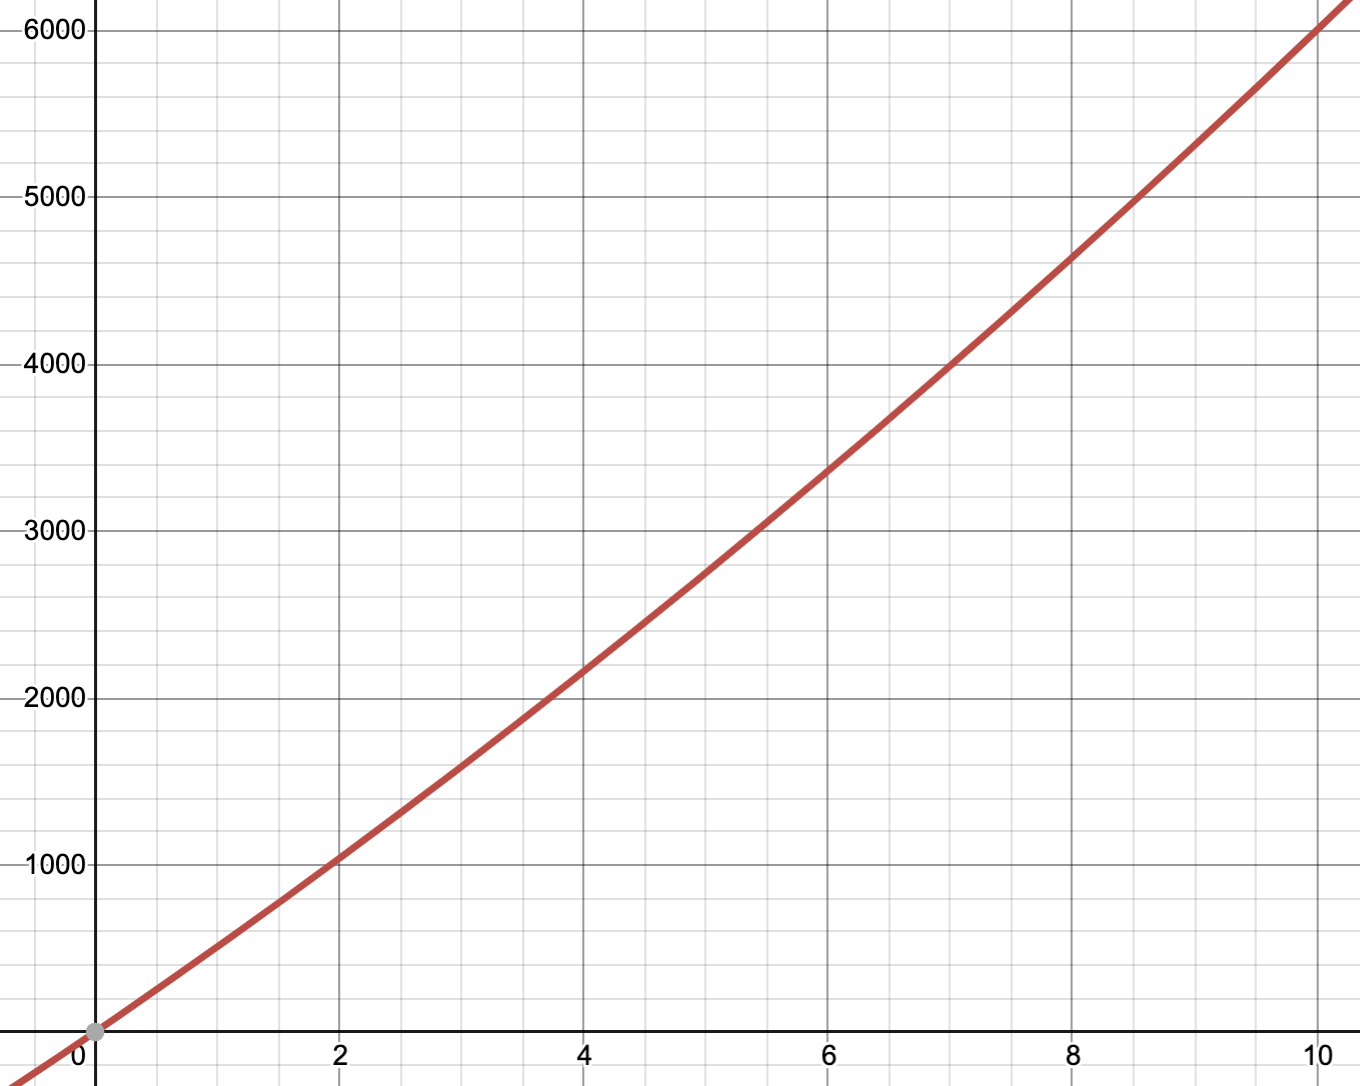
\includegraphics[scale=0.4]{ps5fig5}
\caption{Total cost, 2.4.f.}
\end{figure}
\begin{figure}
\centering
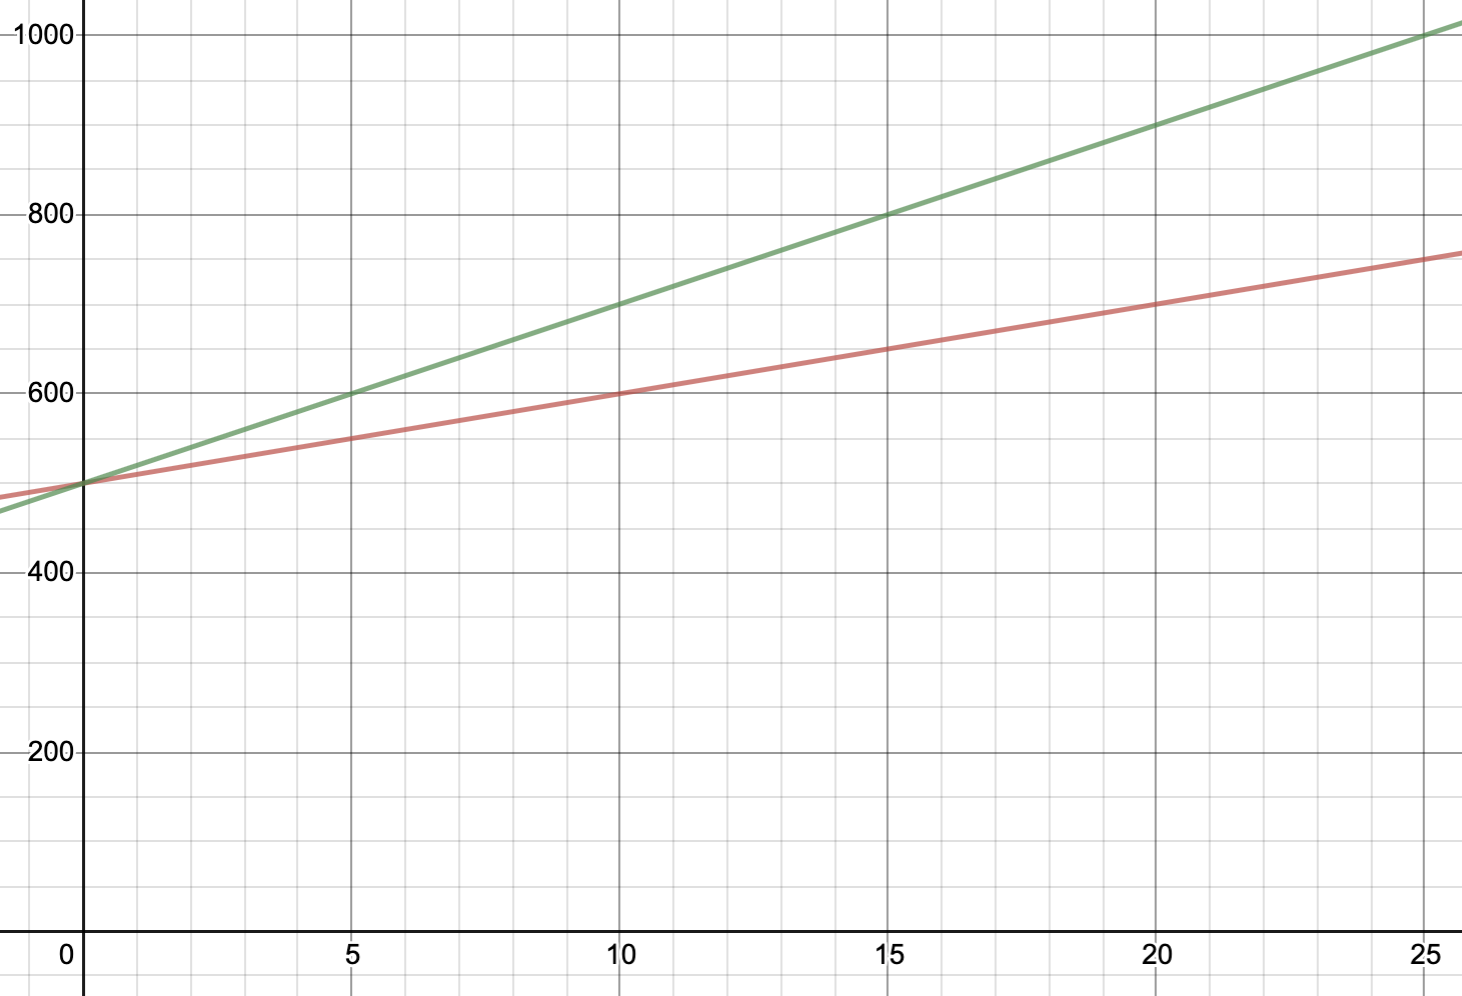
\includegraphics[scale=0.4]{ps5fig6}
\caption{Average cost and marginal cost, 2.4.f. Average cost in red, marginal cost in green.}
\end{figure}
\item See figures 7 and 8. The firm FOC is
\[ p = 2q \]
If $p < 20$, then the firm solution isn't interior and just chooses $q=0$. For $p \ge 20$, we have the interior solution corresponding to the FOC. At equilibrium then, we will have $0$ profits at $p=20$, and each firm will produce $q=10$. The net quantity is then $Q = 1020 - 20 = 1000$, so there are $n=100$ firms in the market. We can interpret the fixed cost $100$ as just being the cost of an indivisible input where the firm only needs one unit of the input to produce. Hence the $100$ can be interpreted into the variable cost, since choosing $q=0$ does not have this cost.
\begin{figure}
\centering
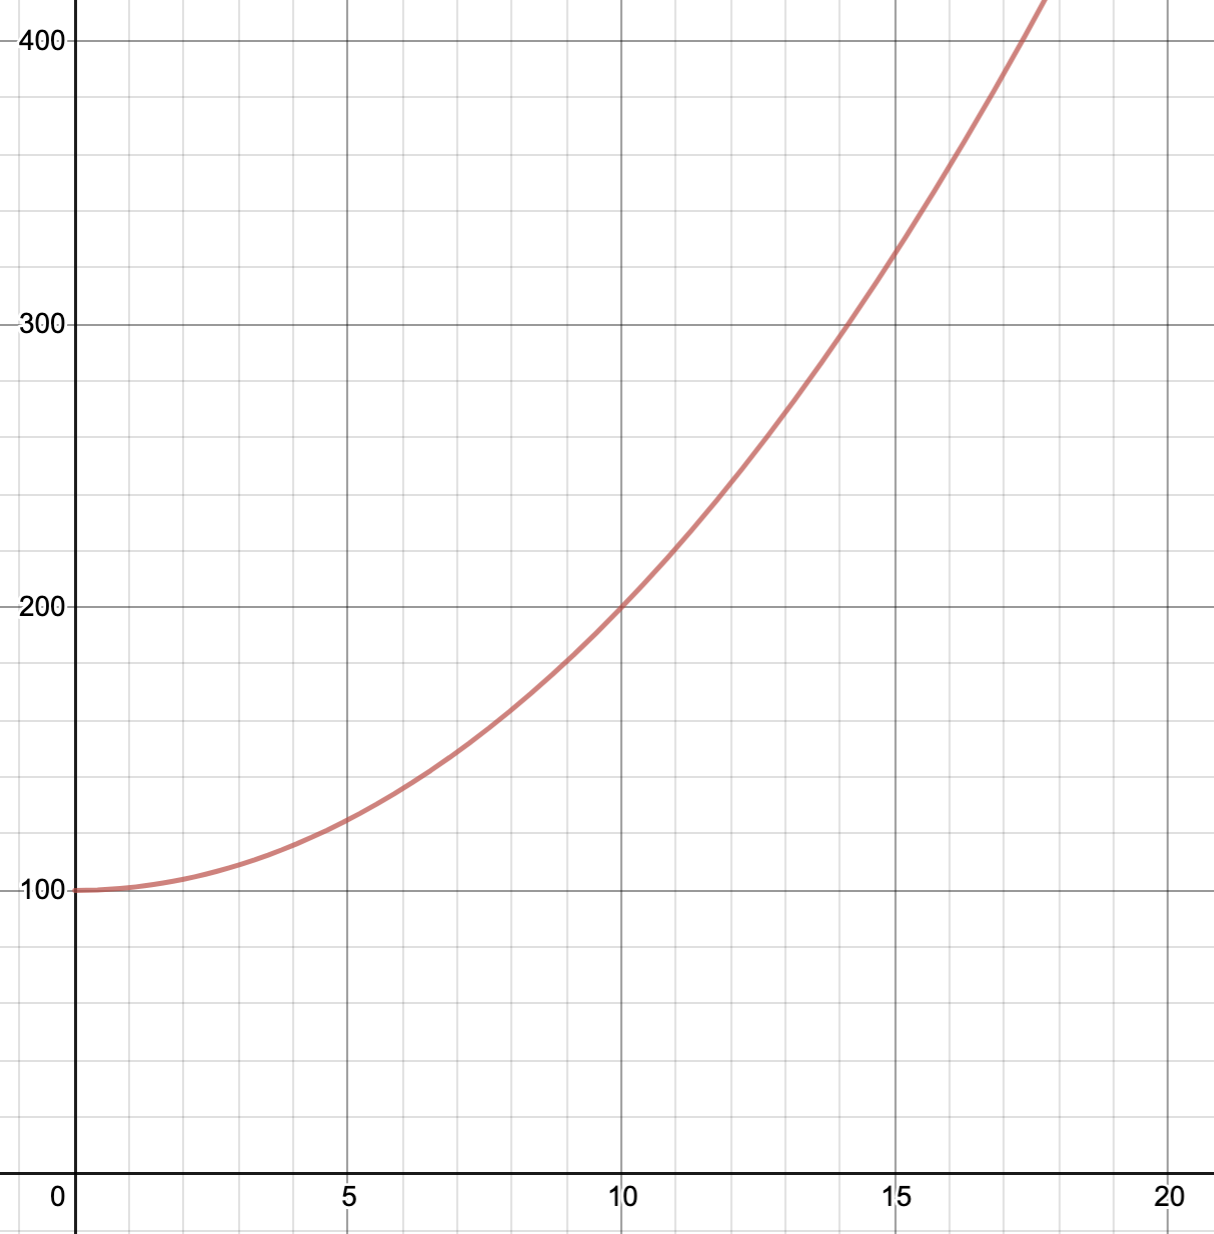
\includegraphics[scale=0.4]{ps5fig7}
\caption{Total cost, 2.4.g.}
\end{figure}
\begin{figure}
\centering
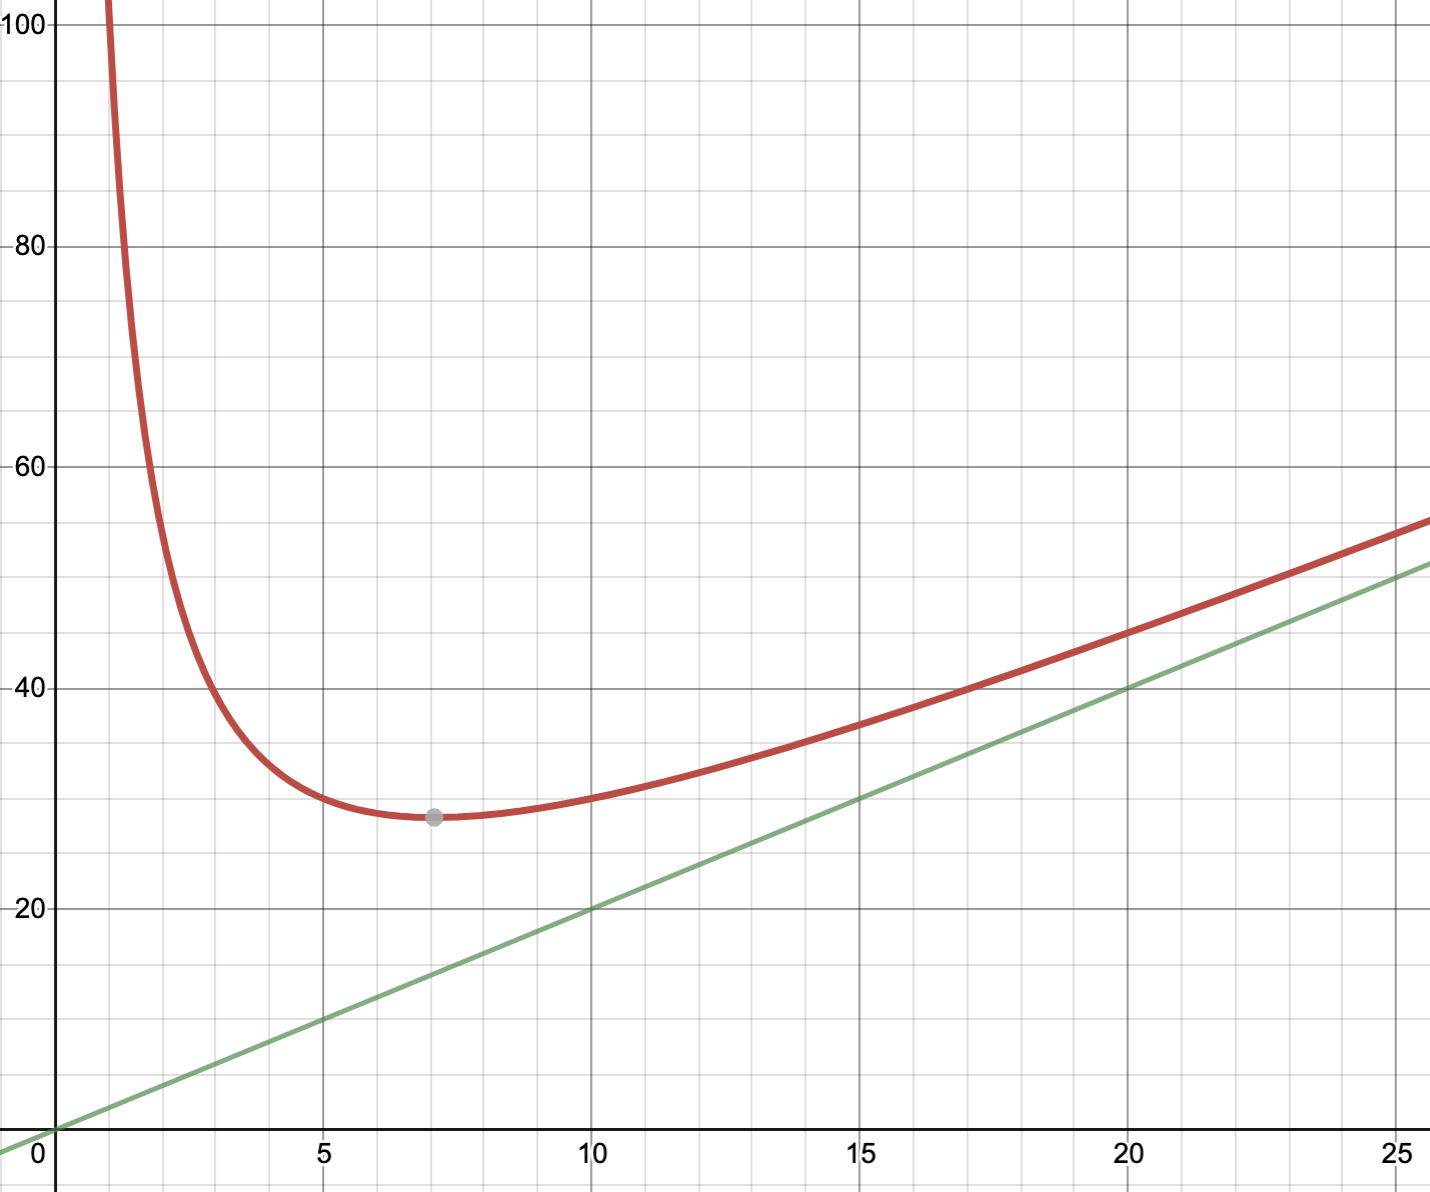
\includegraphics[scale=0.4]{ps5fig8}
\caption{Average cost and marginal cost, 2.4.g. Average cost in red, marginal cost in green.}
\end{figure}
\item This may not even have a solution to the firm maximization. Suppose $p > 1$. Since the marginal cost is 1, the firm would want to produce an arbitrarily large quantity. This is not good for modeling.
\item I'd probably pick the original cubic cost, as the analysis is clean but nontrivial. Admittedly it is slightly disadvantageous in that the production set fails convexity, but better for the purpose of teaching about equilibrium.
\end{itemize}
\end{document}
	% line of code telling latex that your document is ending. If you leave this out, you'll get an error
